\documentclass[11pt]{article}

% ---------- packages ----------
\usepackage[margin=1in]{geometry}
\usepackage{amsmath,amssymb,mathtools}
\usepackage{booktabs}
\usepackage{array}
\usepackage{enumitem}
\usepackage{xcolor}
\usepackage{listings}
\usepackage{hyperref}
\usepackage{tikz}
\usetikzlibrary{arrows.meta, positioning, fit, backgrounds}

% ---------- code listing style ----------
\definecolor{codebg}{RGB}{245,245,245}
\definecolor{codekw}{RGB}{0,90,180}
\lstset{
  language=JavaScript,
  basicstyle=\ttfamily\small,
  keywordstyle=\color{codekw}\bfseries,
  commentstyle=\color{gray}\itshape,
  numbers=none,
  backgroundcolor=\color{codebg},
  frame=single,
  rulecolor=\color{gray!40},
  breaklines=true,
  showstringspaces=false,
  tabsize=2,
  xleftmargin=1em,
  xrightmargin=1em
}

% ---------- tikz styles ----------
\tikzset{
  block/.style={rectangle, draw=black!70, rounded corners, fill=blue!7,
    text width=7.2cm, align=center, minimum height=1.05cm, font=\small},
  data/.style={rectangle, draw=black!60, fill=yellow!12,
    text width=6cm, align=center, minimum height=0.9cm, font=\small\ttfamily},
  decision/.style={diamond, draw=black!70, fill=red!6, aspect=2.4,
    text width=3.4cm, align=center, font=\small},
  arrowline/.style={-{Latex[length=2.2mm]}, thick},
  sidearrow/.style={-{Latex[length=2mm]}, thick, gray!70}
}

% ---------- convenience macros ----------
\newcommand{\code}[1]{\texttt{#1}}
\newcommand{\func}[1]{\texttt{\textbf{#1}}}
\newcommand{\type}[1]{\textsc{#1}}
\newcommand{\R}{\mathbb{R}}

\title{\textbf{Mean Curvature Flow, Traced End to End}\\[2pt]
\large A data-flow blueprint of \code{mean-curvature-flow.js},
\code{modified-mean-curvature-flow.js}, and \code{index.html}}
\author{geometry-processing-js --- \texttt{projects/geometric-flow}}
\date{}

\begin{document}
\maketitle

\vspace{-1.2em}
\begin{center}
\begin{minipage}{0.9\textwidth}
\small
\textbf{How to read this document.} Every function from \code{mean-curvature-flow.js},
\code{modified-mean-curvature-flow.js}, and the inline \code{<script>} in \code{index.html}
is walked in the order the program actually calls it. For each one we record: (1) what
comes \emph{in}, (2) whether a \emph{new object} is created or an existing one is
\emph{mutated in place}, and (3) the linear-algebra / discrete-differential-geometry meaning
of that transformation, written as an equation. The program naturally splits into two
pipelines that share state but do very different jobs:

\begin{itemize}[leftmargin=1.4em]
  \item \textbf{Section A --- the numerical core.} Repeatedly nudge every vertex position
    a small implicit step along the surface Laplacian of the mesh itself --- the discrete
    analogue of flowing a surface in the direction of its mean curvature vector. This is
    pure linear algebra --- no Three.js is involved --- and it mutates the mesh's geometry
    in place, one \func{integrate(h)} call at a time.
  \item \textbf{Section B --- extraction \& visualization.} Turn the (mutated) vertex
    positions into things a GPU can draw: refreshed position/normal buffers, a refreshed
    wireframe overlay, and a dat.gui panel that lets the user pick a flow variant, a time
    step, and fire off one flow step at a time.
\end{itemize}
Both pipelines are kicked off by the same place --- the dat.gui panel's \code{Integrate}
button handler, defined inline in \code{index.html} --- which is the hinge between them
(Section~\ref{sec:bridge}).
\end{minipage}
\end{center}

\tableofcontents

% =====================================================================
\section{Section A --- The Numerical Core: Mean Curvature Flow}
\label{sec:sectionA}
% =====================================================================

\begin{center}
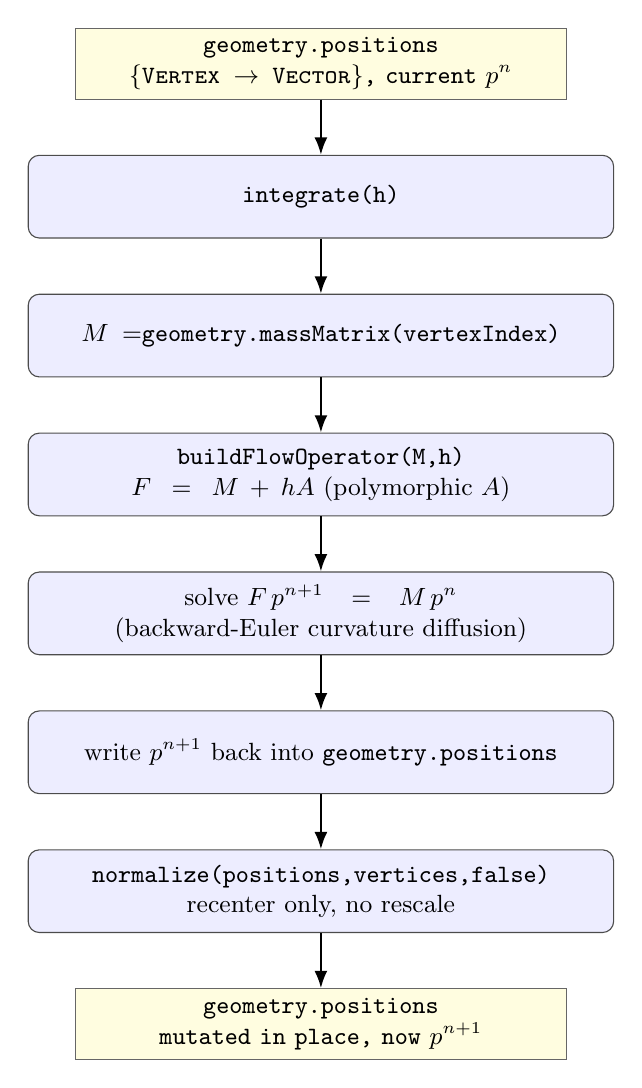
\begin{tikzpicture}[node distance=7mm]
  \node[data] (p0) {\code{geometry.positions}\\ $\{\type{Vertex}\to\type{Vector}\}$, current $p^{n}$};
  \node[block, below=of p0] (integrate) {\func{integrate(h)}};
  \node[block, below=of integrate] (M) {$M=$\func{geometry.massMatrix(vertexIndex)}};
  \node[block, below=of M] (F) {\func{buildFlowOperator(M,h)}\\ $F=M+hA$ (polymorphic $A$)};
  \node[block, below=of F] (solve) {solve $F\,p^{n+1}=M\,p^{n}$\\ (backward-Euler curvature diffusion)};
  \node[block, below=of solve] (write) {write $p^{n+1}$ back into \code{geometry.positions}};
  \node[block, below=of write] (norm) {\func{normalize(positions,vertices,false)}\\ recenter only, no rescale};
  \node[data, below=of norm] (p1) {\code{geometry.positions}\\ mutated in place, now $p^{n+1}$};

  \draw[arrowline] (p0) -- (integrate);
  \draw[arrowline] (integrate) -- (M);
  \draw[arrowline] (M) -- (F);
  \draw[arrowline] (F) -- (solve);
  \draw[arrowline] (solve) -- (write);
  \draw[arrowline] (write) -- (norm);
  \draw[arrowline] (norm) -- (p1);
\end{tikzpicture}
\end{center}

\subsection{Precomputed inputs \& data structures}
\label{sec:precompute}

Both flow classes are built on top of the same combinatorial/geometric foundation that
\code{index.html}'s own \func{initMesh(text)} assembles once per loaded \code{.obj} file
(via \code{MeshIO.readOBJ}, \code{new Mesh()}, \code{mesh.build(polygonSoup)}, and
\code{new Geometry(mesh, polygonSoup["v"])} --- the same halfedge-mesh-plus-embedding
pipeline used throughout \code{geometry-processing-js}). Two details of that foundation
matter specifically for this project:

\begin{itemize}[leftmargin=1.6em]
\item \code{new Geometry(...)} normalizes the freshly loaded mesh by \emph{re-centering and
  rescaling to the unit ball} (rescale defaults to \code{true}). This fixes the initial
  scale so that a single time step \code{h} behaves consistently across different input
  meshes.
\item After that, every \func{integrate(h)} call only \emph{re-centers} the mesh
  (\func{normalize(..., false)}, Section~\ref{sec:integrate}) --- it deliberately does
  \emph{not} rescale back to unit size. Mean curvature flow shrinks a surface over time (a
  sphere shrinks to a point in finite time); allowing that shrinkage to persist across steps
  is exactly what makes the flow visually and numerically meaningful. Rescaling every step
  would fight the flow and hide it.
\end{itemize}

\paragraph{\func{MeanCurvatureFlow} constructor --- \type{mean-curvature-flow.js}}
\textbf{Input:} \code{geometry} : \type{gpGeometry}.\\
\textbf{Output (new object):} \code{this} : \type{MeanCurvatureFlow}, exposing
\code{geometry} and \code{vertexIndex} : $\{\type{Vertex}\to\mathbb{Z}\}$, a dictionary
mapping every vertex object to a unique integer in $[0,V)$, built by the shared global
helper \code{indexElements(geometry.mesh.vertices)}. This index is independent of (though
numerically identical in practice to) each vertex's own \code{.index} field set by
\code{mesh.build}; it exists so every matrix row/column used below can be addressed by
plain array index instead of vertex-object identity.

\paragraph{\func{ModifiedMeanCurvatureFlow} constructor --- \type{modified-mean-curvature-flow.js}}
\textbf{Input:} \code{geometry} : \type{gpGeometry}.\\
\textbf{Output (new object):} \code{this} : \type{ModifiedMeanCurvatureFlow}
(\code{extends MeanCurvatureFlow}), exposing everything the base constructor exposes, plus
one more field:
\begin{lstlisting}
constructor(geometry) {
  super(geometry);
  this.A = geometry.laplaceMatrix(this.vertexIndex);
}
\end{lstlisting}
\code{this.A} : \type{SparseMatrix} $V\times V$ is the cotangent Laplacian evaluated
\emph{once}, at whatever shape the mesh has \emph{at construction time} (i.e.\ the freshly
loaded, undeformed mesh). This one line is the entire substance of the ``modified'' variant
--- see Section~\ref{sec:buildflow} for why it exists and how it changes the flow.

\subsection{\func{buildFlowOperator(M, h)} --- the flow operator, two ways}
\label{sec:buildflow}
\textbf{Input:} \code{M} : \type{SparseMatrix} $V\times V$ (a mass matrix), \code{h} :
\type{number} (the time step). \textbf{Output (new object):} \code{F} : \type{SparseMatrix}
$V\times V$.

\paragraph{Base version --- \func{MeanCurvatureFlow\#buildFlowOperator}.}
\begin{lstlisting}
buildFlowOperator(M, h) {
  let A = this.geometry.laplaceMatrix(this.vertexIndex);

  // F = M + hA
  return M.plus(A.timesReal(h));
}
\end{lstlisting}
Here \code{A} is recomputed \emph{fresh, on every call}, from \code{this.geometry}'s
\emph{current} positions. Because \code{integrate} (Section~\ref{sec:integrate}) mutates
those same positions in place after every step, this recomputation is exactly what lets
the operator track the mesh as it deforms: the cotangent Laplacian
\[
  A_{ij} = -\frac{\cot\alpha_{ij}+\cot\beta_{ij}}{2}\ \ (j\ne i),
  \qquad
  A_{ii} = \varepsilon + \sum_{j\sim i}\frac{\cot\alpha_{ij}+\cot\beta_{ij}}{2},
\]
(with $\varepsilon=10^{-8}$ for positive-definiteness, and the same sign convention as
elsewhere in the library so that $A\approx-\Delta$) depends on the triangle angles
$\alpha_{ij},\beta_{ij}$, which change as the surface moves. The flow operator itself is
\[
  F = M + hA .
\]

\paragraph{Overridden version --- \func{ModifiedMeanCurvatureFlow\#buildFlowOperator}.}
\begin{lstlisting}
buildFlowOperator(M, h) {
  // F = M + hA
  return M.plus(this.A.timesReal(h));
}
\end{lstlisting}
Textually almost identical --- $F=M+hA$ --- but \code{A} is no longer a local variable
rebuilt from \code{this.geometry}; it is \code{this.A}, the matrix cached once in the
constructor from the \emph{original, undeformed} mesh. Every later step reuses that same
fixed matrix no matter how far the surface has since moved.

\paragraph{Why freeze the Laplacian?} This is the idea from the class's second reference
(Kazhdan, Solomon \& Ben-Chen, ``Can Mean-Curvature Flow Be Made Non-Singular?''). As an
ordinary mean curvature flow shrinks a surface, triangles can become thin or obtuse, which
drives some cotangent weights toward $\pm\infty$ and makes the freshly-rebuilt operator
increasingly ill-conditioned --- in the worst case the flow develops a finite-time
singularity (self-intersection or a degenerate, exploded mesh) before it would otherwise
converge. Freezing $A$ at the mesh's original, well-conditioned triangulation keeps the
linear system well-behaved for arbitrarily many steps. The trade-off is exactness: the
``modified'' flow is no longer driven by the mean curvature of the \emph{current} shape,
only by a fixed elliptic operator that approximates it --- a smoothing flow that is provably
non-singular rather than the literal geometric flow.

\paragraph{Dynamic dispatch.} \func{integrate(h)} (Section~\ref{sec:integrate}) is defined
once, on \code{MeanCurvatureFlow}, and always calls \code{this.buildFlowOperator(M, h)}. It
never checks which subclass it is running on --- JavaScript's normal method dispatch means
\code{this.buildFlowOperator} resolves to whichever version (base or overridden) actually
matches the constructed object, so the exact same \func{integrate} body drives both flow
variants.

\subsection{\func{integrate(h)} --- the full backward-Euler step}
\label{sec:integrate}
\textbf{Input:} \code{h} : \type{number} (time step, read from the dat.gui ``Time Step''
slider). \textbf{No new object returned} --- mutates the existing \code{Vector} instances
inside \code{this.geometry.positions} in place, and has no return value.

\begin{lstlisting}
integrate(h) {
  let vertices = this.geometry.mesh.vertices;
  let V = vertices.length;
  let M = this.geometry.massMatrix(this.vertexIndex);
  let F = this.buildFlowOperator(M, h);

  let f0 = DenseMatrix.zeros(V, 3);
  for (let v of vertices) {
    let i = this.vertexIndex[v];
    let p = this.geometry.positions[v];

    f0.set(p.x, i, 0);
    f0.set(p.y, i, 1);
    f0.set(p.z, i, 2);
  }

  let rhs = M.timesDense(f0);

  let llt = F.chol();
  let fh = llt.solvePositiveDefinite(rhs);

  for (let v of vertices) {
    let i = this.vertexIndex[v];
    let p = this.geometry.positions[v];

    p.x = fh.get(i, 0);
    p.y = fh.get(i, 1);
    p.z = fh.get(i, 2);
  }

  normalize(this.geometry.positions, vertices, false);
}
\end{lstlisting}

\begin{enumerate}[leftmargin=1.6em]
\item \textbf{Build the mass matrix.} \code{this.geometry.massMatrix(this.vertexIndex)}
  $\to$ \textbf{new object} \code{M} : \type{SparseMatrix} $V\times V$, the same diagonal
  barycentric-dual-area matrix used throughout the library:
  $M_{ii}=\sum_{f\ni i}\mathrm{area}(f)/3$. Rebuilt fresh every call, since the mesh's
  triangle areas change as it deforms.

\item \textbf{Build the flow operator.} \code{this.buildFlowOperator(M, h)} $\to$
  \textbf{new object} \code{F} : \type{SparseMatrix} $V\times V$ --- see
  Section~\ref{sec:buildflow} for the two possible bodies this resolves to.

\item \textbf{Pack the current positions as a right-hand side.} \code{f0 =
  DenseMatrix.zeros(V, 3)} $\to$ \textbf{new object}, then filled row-by-row so that row $i$
  holds vertex $i$'s current position $(p_i^n)_x,(p_i^n)_y,(p_i^n)_z$. Packing all three
  coordinates as three columns of \emph{one} dense matrix (rather than three separate
  length-$V$ solves) matters below: it lets a single Cholesky factorization be reused for
  all three coordinate channels at once, since $x$, $y$, and $z$ are each governed by the
  exact same operator $F$.

\item \textbf{Form the right-hand side.} \code{M.timesDense(f0)} $\to$ \textbf{new object}
  \code{rhs} : \type{DenseMatrix} $V\times3$, i.e.\ $\mathrm{rhs}=M p^{n}$.

\item \textbf{Factor and solve.} \code{F.chol()} $\to$ \textbf{new object} \code{llt} :
  \type{Cholesky}, a sparse Cholesky factorization $F=LL^{\top}$ (see the heat-method
  blueprint for why Cholesky is the right tool for a symmetric positive-definite system).
  \code{llt.solvePositiveDefinite(rhs)} $\to$ \textbf{new object} \code{fh} :
  \type{DenseMatrix} $V\times3$, solving
  \[
    F\,p^{n+1} \;=\; M\,p^{n}
    \quad\Longleftrightarrow\quad
    (M+hA)\,p^{n+1} = M\,p^{n}.
  \]
  This is exactly the backward-Euler (implicit) discretization of the geometric heat
  equation $\partial p/\partial t=\Delta p$ applied to the \emph{embedding} (position)
  function of the surface instead of to a scalar temperature field:
  \[
    M\,\frac{p^{n+1}-p^{n}}{h} = -A\,p^{n+1}
    \quad\Longleftrightarrow\quad
    (M+hA)\,p^{n+1}=M\,p^{n}.
  \]
  The reason this update moves the surface at all is a classical fact from differential
  geometry: applying the Laplace--Beltrami operator to a surface's position function
  returns (twice) its mean curvature normal, $\Delta p = -2H\mathbf{n}$. So diffusing the
  position field by the surface Laplacian --- exactly what this linear solve does, one
  implicit step at a time --- \emph{is} mean curvature flow: every point moves inward
  fastest wherever the surface is most sharply curved, which is precisely what smooths out
  bumps and eventually collapses closed surfaces. Implicit (backward) Euler is used, rather
  than the simpler explicit forward Euler, because it is unconditionally stable: the cotan
  Laplacian is a stiff operator, and an explicit step would need a vanishingly small $h$ to
  avoid the surface blowing up, whereas the implicit solve above stays stable for the much
  larger $h$ exposed on the dat.gui slider (up to $0.1$).

\item \textbf{Write the new positions back.} Each vertex's existing \code{Vector} object
  (\code{this.geometry.positions[v]}) has its \code{.x},\code{.y},\code{.z} fields
  overwritten from row $i$ of \code{fh}. \emph{The dictionary \code{geometry.positions}
  itself is never reallocated} --- only the numbers inside the \code{Vector} objects it
  already holds change, which is exactly what lets \code{index.html}'s
  \func{updateMesh()} (Section~\ref{sec:updatemesh}) read the result straight back out
  through the same references it already has.

\item \textbf{Re-center.} \func{normalize(this.geometry.positions, vertices, false)}
  (Section~\ref{sec:precompute}) shifts every position by $-\bar p$ where
  $\bar p=\tfrac1V\sum_i p_i^{n+1}$, but --- because the third argument is \code{false} ---
  does \emph{not} rescale back to unit radius, so the flow's characteristic shrinkage
  remains visible from one \code{Integrate} click to the next.
\end{enumerate}

\subsection{Control flow, step by step}
\label{sec:controlflow}
Putting Sections~\ref{sec:precompute}--\ref{sec:integrate} together, one click of the
dat.gui ``Integrate'' button runs exactly this sequence (the branch in step 2 is the only
difference between the two flow variants):

\begin{enumerate}[leftmargin=1.8em]
\item Read the currently selected flow object (\code{meanCurvatureFlow} or
  \code{modifiedMeanCurvatureFlow}, chosen by the ``Method'' dropdown) and call its
  \func{integrate(h)} with the current ``Time Step'' value.
\item Inside \func{integrate}: build $M$ (fresh every call); build $F=M+hA$ via
  \func{buildFlowOperator}, where $A$ is either freshly recomputed from the deformed mesh
  (plain MCF) or the fixed matrix cached at load time (Modified MCF).
\item Pack the current per-vertex positions into a dense $V\times3$ matrix $p^{n}$; form the
  right-hand side $Mp^{n}$.
\item Cholesky-factor $F$ once, then solve $(M+hA)p^{n+1}=Mp^{n}$ for all three coordinate
  columns simultaneously.
\item Overwrite every vertex's stored position in place with the corresponding row of
  $p^{n+1}$.
\item Re-center the whole point set about its new center of mass (no rescale).
\item Control returns to the button handler in \code{index.html}, which frees the
  transient WASM-backed objects created above and hands the (mutated) \code{geometry} off
  to Section~\ref{sec:sectionB} to be redrawn (Section~\ref{sec:bridge}).
\end{enumerate}

% =====================================================================
\section{Section B --- Rendering \& Visualization in \code{index.html}}
\label{sec:sectionB}
% =====================================================================

Section~\ref{sec:sectionA} never touches Three.js, and the code in this section never
touches a \type{SparseMatrix} or \type{DenseMatrix} directly --- it only consumes the
\code{mesh}/\code{geometry} objects (before and after each flow step) and turns their
numbers into buffers a GPU can rasterize, plus the dat.gui plumbing that lets a person
drive the whole thing.

\begin{center}
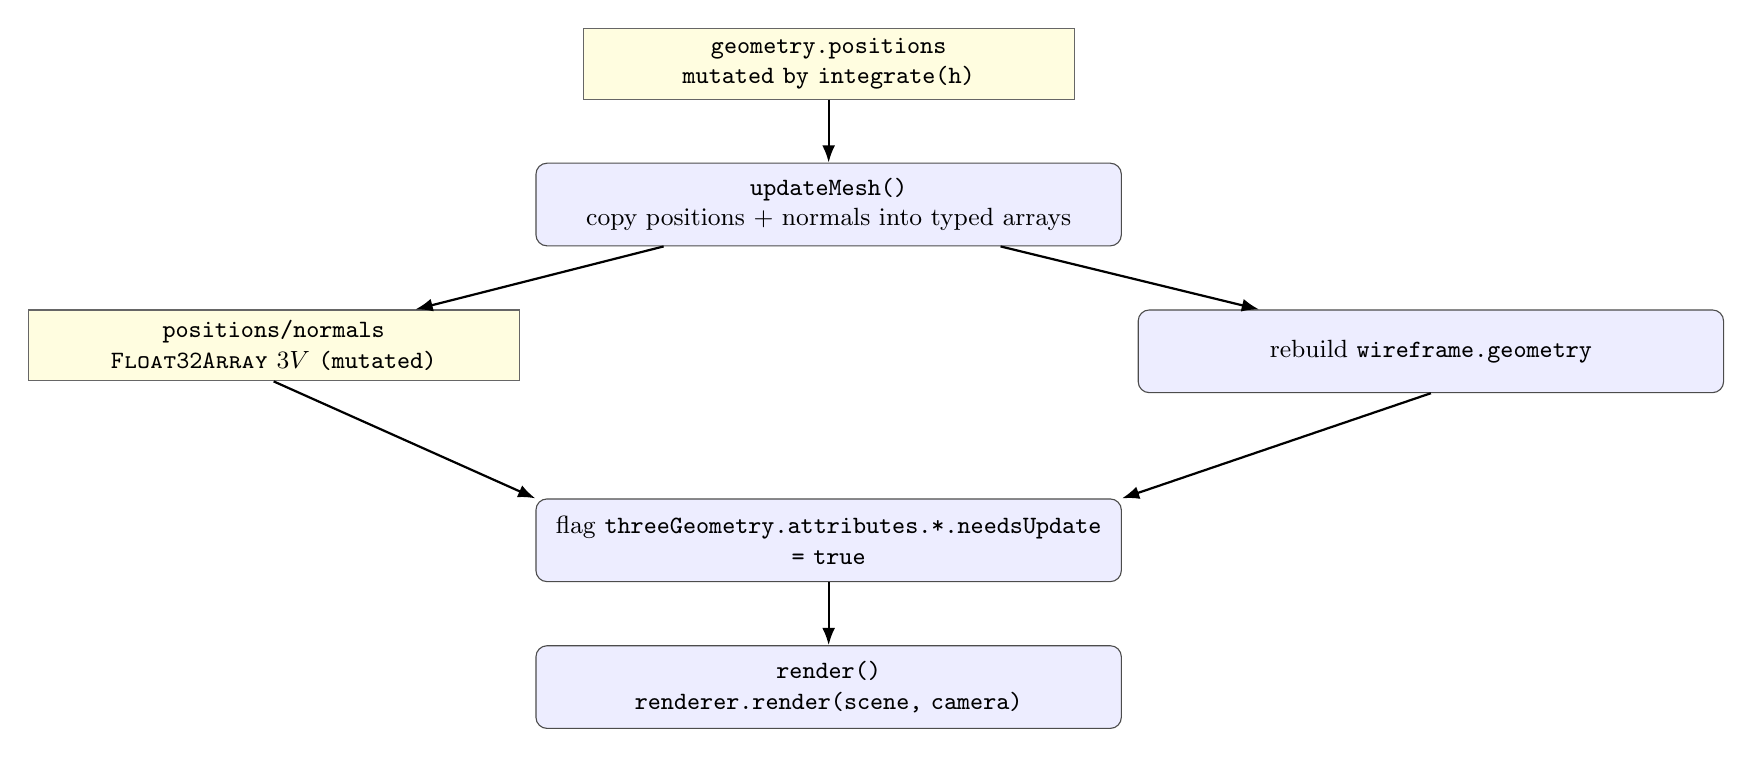
\begin{tikzpicture}[node distance=8mm]
  \node[data] (pos) {\code{geometry.positions}\\ mutated by \func{integrate(h)}};
  \node[block, below=of pos] (update) {\func{updateMesh()}\\ copy positions + normals into typed arrays};
  \node[data, below left=8mm and 2mm of update] (buf) {\code{positions}/\code{normals}\\ \type{Float32Array} $3V$ (mutated)};
  \node[block, below right=8mm and 2mm of update] (wire) {rebuild \code{wireframe.geometry}};
  \node[block, below=32mm of update] (flag) {flag \code{threeGeometry.attributes.*.needsUpdate = true}};
  \node[block, below=of flag] (render) {\func{render()}\\ \code{renderer.render(scene, camera)}};

  \draw[arrowline] (pos) -- (update);
  \draw[arrowline] (update) -- (buf);
  \draw[arrowline] (update) -- (wire);
  \draw[arrowline] (buf.south) -- (flag.north west);
  \draw[arrowline] (wire.south) -- (flag.north east);
  \draw[arrowline] (flag) -- (render);
\end{tikzpicture}
\end{center}

\subsection{Page \& scene scaffolding}
\label{sec:scaffolding}
These functions are ordinary Three.js setup, run once from \func{init()} and largely
independent of the flow math: \func{initRenderer(container)} creates a
\code{THREE.WebGLRenderer}, sets its pixel ratio and size, and appends its canvas to the
page; \func{initCamera()} builds a perspective camera; \func{initScene()} creates the
\code{THREE.Scene} and its background color; \func{initLights()} adds an ambient light and
a point light, both parented to the \emph{camera} (so they move with the viewer rather than
sitting fixed in world space) before the camera itself is added to the scene;
\func{initControls()} wraps the canvas in a \code{THREE.TrackballControls} (this project
vendors Three.js r87 with its own classic-script control scheme, not this site's
\code{ArcballControls}); and \func{addEventListeners()}/\func{onWindowResize()} keep the
camera aspect ratio, renderer size, and controls in sync with the browser window.

\subsection{\func{initThreeMesh()} --- building the drawable buffers}
\label{sec:initthreemesh}
\textbf{Input:} none (reads outer-scope \code{mesh}, \code{geometry}). \textbf{New
objects:} \code{threeGeometry} : \type{THREE.BufferGeometry}; \code{threeMesh} :
\type{THREE.Mesh}; \code{wireframe} : \type{THREE.LineSegments}; plus the flat typed
arrays \code{positions}, \code{normals}, \code{colors} : \type{Float32Array} of length
$3V$, and \code{indices} : \type{Uint32Array} of length $3F$.

For every vertex $v$ with index $i$, this copies \code{geometry.positions[v]} and
\code{geometry.vertexNormalEquallyWeighted(v)} into flat position/normal buffers at offset
$3i$, and initializes every vertex's color to a flat \code{ORANGE} (unlike the heat-method
project, geometric flow never drives vertex color from a scalar field --- color stays
constant throughout, since the thing being visualized is a change in \emph{shape}, not a
scalar quantity defined on a fixed shape). For every face it writes the three corner
indices into \code{indices}. These buffers are attached to \code{threeGeometry} as
\code{BufferAttribute}s, and a \code{THREE.MeshPhongMaterial} is built with
\code{vertexColors: THREE.VertexColors}, \code{side: THREE.DoubleSide}, and a small
\code{polygonOffset} (so the filled triangles are pushed slightly behind the wireframe
overlay in depth, preventing z-fighting between the two coincident surfaces). A separate
\code{wireframe} \code{THREE.LineSegments} is built from
\code{new THREE.WireframeGeometry(threeGeometry)} and a black \code{LineBasicMaterial}, and
\func{toggleWireframe(showWireframe)} is called once to sync its initial visibility with
the GUI checkbox. \textbf{The important detail for Section B:} \code{positions},
\code{normals}, and \code{indices} are kept as live outer-scope arrays and attributes on
\code{threeGeometry}, so \func{updateMesh()} (Section~\ref{sec:updatemesh}) can overwrite
them in place after every flow step instead of rebuilding the mesh from scratch.

\subsection{\func{initMesh(text)} (index.html) --- the load pipeline}
\label{sec:initmesh-page}
\textbf{Input:} \code{text} : \type{string}, raw \code{.obj} file contents (the bundled
\code{bunny} template string on startup, or a user-uploaded file's text via the
\code{fileInput}/\code{FileReader} listener registered in \code{window.onload}).
\textbf{Effect:} no return value; (re)assigns the outer-scope \code{mesh}, \code{geometry},
\code{threeMesh}, \code{meanCurvatureFlow}, and \code{modifiedMeanCurvatureFlow}.

\begin{lstlisting}
function initMesh(text) {
  let polygonSoup = MeshIO.readOBJ(text);
  mesh = new Mesh();
  if (mesh.build(polygonSoup)) {
    scene.remove(threeMesh);
    memoryManager.deleteExcept([]);

    geometry = new Geometry(mesh, polygonSoup["v"]);

    initThreeMesh();
    scene.add(threeMesh);

    meanCurvatureFlow = new MeanCurvatureFlow(geometry);
    modifiedMeanCurvatureFlow = new ModifiedMeanCurvatureFlow(geometry);
    ...
  }
}
\end{lstlisting}
This mirrors the parse/build/embed pipeline described in Section~\ref{sec:precompute}, then
does three things specific to this project: it removes any previously displayed mesh from
the scene and frees \emph{every} WASM-backed object from the previous mesh
(\code{memoryManager.deleteExcept([])}, an empty keep-list, since a brand-new mesh makes the
old flow operators meaningless); it rebuilds the drawable Three.js mesh
(Section~\ref{sec:initthreemesh}); and it constructs \emph{both} flow objects up front ---
\code{new MeanCurvatureFlow(geometry)} and \code{new ModifiedMeanCurvatureFlow(geometry)}
--- against the same freshly loaded \code{geometry}, even though only one of them will ever
be driven by a given ``Integrate'' click. Building both immediately is what lets
\code{modifiedMeanCurvatureFlow}'s cached \code{this.A} (Section~\ref{sec:precompute}) be
captured from the mesh's original, undeformed shape, and what lets the ``Method'' dropdown
switch between the two variants instantly with no rebuild cost later.

\subsection{\func{initGUI()} and the \code{Integrate} bridge}
\label{sec:bridge}
\func{initGUI()} wires a dat.gui panel to five actions/fields: \code{Load Mesh} (clicks
the hidden \code{fileInput}, whose \code{change} listener in \code{window.onload} reads the
chosen \code{.obj} file with a \code{FileReader} and calls
\func{initMesh(reader.result)}); \code{Export Mesh} (serializes the current mesh with
\code{MeshIO.writeOBJ} and hands the text to \func{exportFile}, which builds a throwaway
\code{<a download>} element with a \code{data:} URI, clicks it to trigger a browser
download, and removes it); the \code{Method} dropdown (\code{"MCF"} / \code{"Modified
MCF"}, read --- not reactively watched --- at click time); the \code{Time Step} slider
(bound via \code{.onChange(updateTimeStep)}, so moving it just sets the outer-scope
\code{h}); and \code{Show Wireframe} (bound via \code{.onChange(toggleWireframe)}).

The \code{Integrate} field is the one place Section~\ref{sec:sectionA} and
Section~\ref{sec:sectionB} are called back to back:
\begin{lstlisting}
"Integrate": function() {
  if (this.Method === "MCF") meanCurvatureFlow.integrate(h);
  else modifiedMeanCurvatureFlow.integrate(h);

  memoryManager.deleteExcept([modifiedMeanCurvatureFlow.A]);
  updateMesh();
}
\end{lstlisting}
\begin{enumerate}[leftmargin=1.6em]
\item \textbf{Run Section A.} Depending on the \code{Method} dropdown, exactly one flow
  object's \func{integrate(h)} (Section~\ref{sec:integrate}) is called, mutating
  \code{geometry.positions} in place.
\item \textbf{Free WASM heap memory.} \type{SparseMatrix}/\type{DenseMatrix}/\type{Cholesky}
  instances live in the emscripten/WASM linear-memory heap and are not garbage-collected by
  the JS engine, so every call to \func{integrate} leaks memory unless it is explicitly
  freed. \code{memoryManager.deleteExcept([modifiedMeanCurvatureFlow.A])} frees every other
  WASM-backed object allocated during the call just made (the mass matrix, the flow
  operator, the Cholesky factorization, the packed right-hand side, the solved positions)
  while explicitly preserving \code{modifiedMeanCurvatureFlow.A} --- the one matrix that
  must persist across every future click regardless of which \code{Method} is currently
  selected, since it is only ever built once (Section~\ref{sec:precompute}) and would
  otherwise be silently reclaimed the next time this line runs.
\item \textbf{Run Section B.} \func{updateMesh()} (Section~\ref{sec:updatemesh}) pushes the
  now-updated \code{geometry.positions} into the GPU-visible buffers, unconditionally, every
  click.
\end{enumerate}

\subsection{\func{updateMesh()} --- pushing new positions to the GPU}
\label{sec:updatemesh}
\textbf{Input:} none (reads outer-scope \code{mesh}, \code{geometry}). \textbf{No new
object returned} --- mutates the existing \code{positions}/\code{normals}
\type{Float32Array}s created in \func{initThreeMesh()}, flips two
\code{needsUpdate} flags, and replaces \code{wireframe.geometry}.

\begin{lstlisting}
function updateMesh() {
  for (let v of mesh.vertices) {
    let i = v.index;

    let position = geometry.positions[v];
    positions[3 * i + 0] = position.x;
    positions[3 * i + 1] = position.y;
    positions[3 * i + 2] = position.z;

    let normal = geometry.vertexNormalEquallyWeighted(v);
    normals[3 * i + 0] = normal.x;
    normals[3 * i + 1] = normal.y;
    normals[3 * i + 2] = normal.z;
  }

  threeGeometry.attributes.position.needsUpdate = true;
  threeGeometry.attributes.normal.needsUpdate = true;
  wireframe.geometry = new THREE.WireframeGeometry(threeGeometry);
}
\end{lstlisting}
This is the same copy loop as \func{initThreeMesh()}'s position/normal fill
(Section~\ref{sec:initthreemesh}), but run against the \emph{same} already-allocated
\code{positions}/\code{normals} arrays rather than freshly allocated ones --- each entry is
simply overwritten with the vertex's post-flow position and freshly recomputed
area-weighted vertex normal. Setting \code{threeGeometry.attributes.position.needsUpdate}
and \code{.normal.needsUpdate} to \code{true} is what tells Three.js to re-upload those
\code{BufferAttribute}s to the GPU on the next \func{render()} call, instead of assuming
the buffers are unchanged. The one piece that \emph{cannot} be updated in place is the
wireframe: \code{THREE.WireframeGeometry} bakes a derived, non-indexed edge list out of
\code{threeGeometry} once at construction time and exposes no mechanism to refresh that
derived buffer from a mutated source, so \code{wireframe.geometry} is simply replaced with
a brand-new \code{WireframeGeometry} built from the just-updated \code{threeGeometry} every
time.

\subsection{Minor UI glue}
\func{updateTimeStep(value)} is a one-line setter (\code{h = value}) invoked by the
\code{Time Step} slider's \code{onChange}. \func{toggleWireframe(checked)} adds or removes
the \code{wireframe} \code{LineSegments} as a child of \code{threeMesh} depending on the
\code{Show Wireframe} checkbox. \func{exportFile(text)} and the \code{fileInput} /
\code{FileReader} listener registered in \code{window.onload} implement the OBJ
load/export round trip described in Section~\ref{sec:bridge}. None of these touch
\code{geometry} or either flow object; they only exist to let the dat.gui panel drive the
functions described above.

\subsection{\func{animate()} / \func{render()} --- the draw loop}
\func{animate()} is registered once via \code{requestAnimationFrame} and re-schedules
itself every frame, calling \code{controls.update()} (to advance
\code{TrackballControls}'s momentum/damping) followed by \func{render()}
(\code{renderer.render(scene, camera)}). This loop runs continuously regardless of whether
a flow step just happened --- it simply redraws whatever \code{threeGeometry}'s attributes
currently hold, which is why \func{updateMesh()} only needs to flag \code{needsUpdate} and
never needs to call \func{render()} itself.

\subsection*{Summary table}
\begin{center}
\small
\renewcommand{\arraystretch}{1.3}
\begin{tabular}{@{}p{3.6cm}p{4.7cm}p{4.8cm}@{}}
\toprule
\textbf{Function} & \textbf{Input $\to$ Output / mutation} & \textbf{Role} \\
\midrule
\multicolumn{3}{@{}l}{\textit{Section A --- numerical core (Section~\ref{sec:sectionA})}} \\
\func{MeanCurvatureFlow ctor} & \type{gpGeometry} $\to$ \type{MeanCurvatureFlow} & store geometry, build \code{vertexIndex} \\
\func{ModifiedMeanCurvatureFlow ctor} & \type{gpGeometry} $\to$ \type{ModifiedMeanCurvatureFlow} & as above, plus cache \code{A} once \\
\func{buildFlowOperator} (base) & $M,h\to F$ (new \type{SparseMatrix}) & $F=M+hA$, $A$ recomputed from current shape \\
\func{buildFlowOperator} (override) & $M,h\to F$ (new \type{SparseMatrix}) & $F=M+hA$, $A$ fixed at load time \\
\func{integrate} & $h$ mutates \code{geometry.positions} & one implicit mean-curvature-flow step \\
\midrule
\multicolumn{3}{@{}l}{\textit{Section B --- extraction \& visualization (Section~\ref{sec:sectionB})}} \\
\func{initThreeMesh} & mesh, geometry $\to$ \type{THREE.BufferGeometry}/\type{Mesh}/\type{LineSegments} & drawable surface + position/normal/color buffers \\
\func{initMesh} (index.html) & OBJ text $\to$ mutates \code{mesh},\code{geometry},flow objects & load, embed, and re-arm the two flow variants \\
\func{initGUI} & --- $\to$ dat.gui panel & wires IO, method, time step, integrate, wireframe controls \\
\func{updateMesh} & --- mutates \code{positions}/\code{normals} buffers, \code{wireframe} & push post-flow geometry to the GPU \\
\func{toggleWireframe} & \type{boolean} mutates \code{threeMesh} children & show/hide wireframe overlay \\
\func{exportFile} & text $\to$ triggers a file download & OBJ export \\
\func{animate}/\func{render} & --- $\to$ draws the frame & continuous draw loop \\
\midrule
\code{Integrate} handler & GUI click $\to$ orchestrates both sections & bridge: click $\to$ Section A $\to$ free WASM $\to$ Section B \\
\bottomrule
\end{tabular}
\end{center}

\end{document}
